\documentclass[journal,12pt,twocolumn]{IEEEtran}
%
\usepackage{setspace}
\usepackage{gensymb}
\usepackage{xcolor}
\usepackage{caption}
\usepackage{chngcntr}
%\usepackage{subcaption}
%\doublespacing
\singlespacing
\usepackage{multicol}
%\usepackage{graphicx}
%\usepackage{amssymb}
%\usepackage{relsize}
\usepackage[cmex10]{amsmath}
\usepackage{mathtools}
%\usepackage{amsthm}
%\interdisplaylinepenalty=2500
%\savesymbol{iint}
%\usepackage{txfonts}
%\restoresymbol{TXF}{iint}
%\usepackage{wasysym}
\usepackage{amsthm}
\usepackage{mathrsfs}
\usepackage{txfonts}
\usepackage{stfloats}
\usepackage{cite}
\usepackage{cases}
\usepackage{subfig}
%\usepackage{xtab}
\usepackage{longtable}
\usepackage{multirow}
%\usepackage{algorithm}
%\usepackage{algpseudocode}
\usepackage{enumerate}
\usepackage{mathtools}
\usepackage{iithtlc}
%\usepackage[framemethod=tikz]{mdframed}
\usepackage{listings}
    \usepackage[latin1]{inputenc}                                 %%
    \usepackage{color}                                            %%
    \usepackage{array}                                            %%
    \usepackage{longtable}                                        %%
    \usepackage{calc}                                             %%
    \usepackage{multirow}                                         %%
    \usepackage{hhline}                                           %%
    \usepackage{ifthen}                                           %%
  %optionally (for landscape tables embedded in another document): %%
    \usepackage{lscape}     

%\usepackage{stmaryrd}


%\usepackage{wasysym}
%\newcounter{MYtempeqncnt}
\DeclareMathOperator*{\Res}{Res}
%\renewcommand{\baselinestretch}{2}
\renewcommand\thesection{\arabic{section}}
\renewcommand\thesubsection{\thesection.\arabic{subsection}}
\renewcommand\thesubsubsection{\thesubsection.\arabic{subsubsection}}

\renewcommand\thesectiondis{\arabic{section}}
\renewcommand\thesubsectiondis{\thesectiondis.\arabic{subsection}}
\renewcommand\thesubsubsectiondis{\thesubsectiondis.\arabic{subsubsection}}

% correct bad hyphenation here
\hyphenation{op-tical net-works semi-conduc-tor}

\def\inputGnumericTable{}  

\lstset{
language=python,
frame=single, 
breaklines=true
}
\newcommand\bigzero{\makebox(0,0){\text{\huge0}}}
%\lstset{
	%%basicstyle=\small\ttfamily\bfseries,
	%%numberstyle=\small\ttfamily,
	%language=Octave,
	%backgroundcolor=\color{white},
	%%frame=single,
	%%keywordstyle=\bfseries,
	%%breaklines=true,
	%%showstringspaces=false,
	%%xleftmargin=-10mm,
	%%aboveskip=-1mm,
	%%belowskip=0mm
%}

%\surroundwithmdframed[width=\columnwidth]{lstlisting}


\begin{document}
%

\theoremstyle{definition}
\newtheorem{theorem}{Theorem}[section]
\newtheorem{problem}{Problem}
\newtheorem{proposition}{Proposition}[section]
\newtheorem{lemma}{Lemma}[section]
\newtheorem{corollary}[theorem]{Corollary}
\newtheorem{example}{Example}[section]
\newtheorem{definition}{Definition}[section]
%\newtheorem{algorithm}{Algorithm}[section]
%\newtheorem{cor}{Corollary}
\newcommand{\BEQA}{\begin{eqnarray}}
\newcommand{\EEQA}{\end{eqnarray}}
\newcommand{\define}{\stackrel{\triangle}{=}}

\bibliographystyle{IEEEtran}
%\bibliographystyle{ieeetr}

\providecommand{\nCr}[2]{\,^{#1}C_{#2}} % nCr
\providecommand{\nPr}[2]{\,^{#1}P_{#2}} % nPr
\providecommand{\mbf}{\mathbf}
\providecommand{\pr}[1]{\ensuremath{\Pr\left(#1\right)}}
\providecommand{\qfunc}[1]{\ensuremath{Q\left(#1\right)}}
\providecommand{\sbrak}[1]{\ensuremath{{}\left[#1\right]}}
\providecommand{\lsbrak}[1]{\ensuremath{{}\left[#1\right.}}
\providecommand{\rsbrak}[1]{\ensuremath{{}\left.#1\right]}}
\providecommand{\brak}[1]{\ensuremath{\left(#1\right)}}
\providecommand{\lbrak}[1]{\ensuremath{\left(#1\right.}}
\providecommand{\rbrak}[1]{\ensuremath{\left.#1\right)}}
\providecommand{\cbrak}[1]{\ensuremath{\left\{#1\right\}}}
\providecommand{\lcbrak}[1]{\ensuremath{\left\{#1\right.}}
\providecommand{\rcbrak}[1]{\ensuremath{\left.#1\right\}}}
\theoremstyle{remark}
\newtheorem{rem}{Remark}
\newcommand{\sgn}{\mathop{\mathrm{sgn}}}
\providecommand{\abs}[1]{\left\vert#1\right\vert}
\providecommand{\res}[1]{\Res\displaylimits_{#1}} 
\providecommand{\norm}[1]{\lVert#1\rVert}
\providecommand{\mtx}[1]{\mathbf{#1}}
\providecommand{\mean}[1]{E\left[ #1 \right]}
\providecommand{\fourier}{\overset{\mathcal{F}}{ \rightleftharpoons}}
%\providecommand{\hilbert}{\overset{\mathcal{H}}{ \rightleftharpoons}}
\providecommand{\system}{\overset{\mathcal{H}}{ \longleftrightarrow}}
	%\newcommand{\solution}[2]{\textbf{Solution:}{#1}}
\newcommand{\solution}{\noindent \textbf{Solution: }}
\providecommand{\dec}[2]{\ensuremath{\overset{#1}{\underset{#2}{\gtrless}}}}
%\numberwithin{equation}{subsection}
\numberwithin{equation}{section}
%\numberwithin{equation}{problem}
%\numberwithin{problem}{subsection}
\numberwithin{problem}{section}
\counterwithin{table}{problem}
%\numberwithin{definition}{subsection}
\makeatletter
\@addtoreset{figure}{problem}
\makeatother
%\makeatletter
%\@addtoreset{table}{problem}
%\makeatother

\let\StandardTheFigure\thefigure
%\let\StandardTheTable\thetable
%\renewcommand{\thefigure}{\theproblem.\arabic{figure}}
\renewcommand{\thefigure}{\theproblem}
%\renewcommand{\thetable}{\theproblem}
%\numberwithin{figure}{section}

%\numberwithin{figure}{subsection}

\def\putbox#1#2#3{\makebox[0in][l]{\makebox[#1][l]{}\raisebox{\baselineskip}[0in][0in]{\raisebox{#2}[0in][0in]{#3}}}}
     \def\rightbox#1{\makebox[0in][r]{#1}}
     \def\centbox#1{\makebox[0in]{#1}}
     \def\topbox#1{\raisebox{-\baselineskip}[0in][0in]{#1}}
     \def\midbox#1{\raisebox{-0.5\baselineskip}[0in][0in]{#1}}

%\vspace{3cm}

\title{
\logo{
Gate Problems on Signals and Systems
}
}
%\centering \textbf{\Large Optimization}\\
%\bigskip
%\author{D Hemanth Kumar and G V V Sharma$^{*}$% <-this % stops a space
%\thanks{* The authors are with the Department
%of Electrical Engineering, Indian Institute of Technology, Hyderabad
%502285 India e-mail:  gadepall@iith.ac.in.}% <-this % stops a space
%\thanks{J. Doe and J. Doe are with Anonymous University.}% <-this % stops a space
%\thanks{Manuscript received April 19, 2005; revised January 11, 2007.}}
%}
%
\maketitle

%\tableofcontents

\bigskip
\begin{abstract}
These problems have been selected from GATE question papers and can be used for conducting
tutorials in courses related to Signal Processing.
\end{abstract}


\begin{enumerate}[1.]
\setlength\itemsep{2em}
\item The trigonometric Fourier series of an even function of time does not have the\\

\begin{enumerate}[(A)]
\begin{multicols}{2}
\setlength\itemsep{1em}

\item dc term
\item cosine terms
\item sine terms
\item odd hormonic terms
\end{multicols}
\end{enumerate}

\item The Fourier transform of a real valued time signal\\

\begin{enumerate}[(A)]
\setlength\itemsep{2em}

\item odd symmetry
\item even symmetry
\item conjugate symmetry
\item no symmetry

\end{enumerate}

\item The function $f(t)$ has the Fourier transform $g(w)$. The Fourier Transform

\begin{enumerate}[(A)]
\begin{multicols}{2}
\setlength\itemsep{1em}

\item $\dfrac{1}{2\pi}f(w)$
\item $\dfrac{1}{2\pi}f(-w)$
\item $2\pi f(-w)$
\item None of the above

\end{multicols}
\end{enumerate}

\item The Laplace Transform of $e^{\alpha t}{cos{\alpha t} u(t)}$\\
\begin{enumerate}[(A)]
\begin{multicols}{2}
%\setlength\itemsep{2em}

\item $\dfrac{(s-\alpha)}{(s-\alpha)^{2}+{\alpha}^{2}}$
\item $\dfrac{(s+\alpha)}{(s-\alpha)^{2}+{\alpha}^{2}}$
\item $\dfrac{1}{(s-\alpha)^{2}}$
\item None of the above

\end{multicols}
\end{enumerate}

\item A deterministic signal has the power spectrum given in the figure is, The minimum sampling rate needed to completely represent this signal is\\
\begin{enumerate}[(A)]
\begin{multicols}{2}
\setlength\itemsep{1em}

\item 1 kHz
\item 2 kHz
\item 3 kHz
\item None of the above

\end{multicols}
\end{enumerate}

\item If the Fourier Transform of deterministic signal $g(t)$ is $G(f)$,then \newline \textbf{1.} The fourier Transform of $g(t-2)$ is.\\
        (a) $G(f)e^{-j(4\pi f)}$
       \newline \textbf{2.} The fourier Transform of $g(\dfrac{t}{2})$ is.\\
  			  (b) $G(2f)$
              (c) $2G(2f)$
              (d) $G(f-2)$

\item The transfer function of a system is given by $H(s)=\dfrac{1}{s^{2}(s-2)}$.The impulse response of the system is :( * denotes convolution,and $U(t)$ is unit step function)

\begin{enumerate}[(A)]
\begin{multicols}{2}
\setlength\itemsep{1em}

\item $(t^{2}*e^{-2t})U(t)
$
\item $
(t *e^{2t})U(t)
$
\item $(te^{-2}t)U(t)
$
\item $
(te^{-2t})U(t)
$

\end{multicols}
\end{enumerate}


\item Let $\delta(t)$ denote the delta function.The value of the integral $\int_{-\infty}^{+\infty} \delta(t) cos(\frac{3t}{2}) dt$ is\\

\begin{enumerate}[(A)]
\begin{multicols}{4}
\setlength\itemsep{1em}

\item 1
\item -1
\item 0
\item $\dfrac{\pi}{2}$

\end{multicols}
\end{enumerate}


\item A band limited signal is sampled at the Nyquist rate.The signal can be recovered by passing the samples through\\

\begin{enumerate}[(A)]

\setlength\itemsep{1em}

\item An RC filter
\item an envelope detector
\item a PLL
\item an ideal low-pass filter with appripriate bandwidth


\end{enumerate}

\item The impulse response functions of four linear systems $S_1$,$S_2$,$S_3$ and $S_4$ are given respectively by
\newline $h_1(t)=1$, $h_2(t)=u(t)$,$h_3(t)=\frac{u(t)}{t+1}$, $h_4(t)=e^{-3t}u(t)$.Where $u(t)$ is the unit step function. Which of these systems is time invariant,causal and Stable ?
\begin{enumerate}[(A)]
\begin{multicols}{4}
\setlength\itemsep{1em}

\item $S_1$
\item $S_2$
\item $S_3$
\item $S_4$

\end{multicols}
\end{enumerate}

\item The open-loop DC gain of a unity negative feedback system with close-loop transfer function $\dfrac{s+4}{s^{2}+7s+13}$ is\\
\begin{enumerate}[(A)]
\begin{multicols}{4}
\setlength\itemsep{1em}

\item $\dfrac{4}{13}$
\item $\dfrac{4}{13}$
\item $4$
\item $13$

\end{multicols}
\end{enumerate}

\item The Nyquist sampling interval,for the signal $Sinc(700t)+Sinc(500t)$ is ( in seconds)

\begin{enumerate}[(A)]
\begin{multicols}{4}
\setlength\itemsep{1em}

\item $
\dfrac{1}{350}
$

\item $
\dfrac{\pi}{350} 
$

\item $
\dfrac{1}{700} 
$

\item $
\dfrac{\pi}{175} 
$

\end{multicols}
\end{enumerate}

\item Which of the following cannot be the Fourier series of a periodic signal ?\\
\begin{enumerate}[(A)]
%\begin{multicols}{2}
\setlength\itemsep{1em}

\item $
x(t)=2cos t + 3 cos 3t
$
\item $
x(t)=2 cos \pi t+7 cos t
$
\item $
x(t)=cos t +0.5
$
\item $
x(t)=2 cos 1.5\pi t +sin 3.5 \pi t
$
%\end{multicols}
\end{enumerate}

\item The fourier transform $F(e^{-1}u(t))$ is equal to $\dfrac{1}{a+j2\pi f}$.Therefore,$F\{\dfrac{1}{a+j2\pi t}\}$\\
\begin{enumerate}[(A)]
\begin{multicols}{2}
\setlength\itemsep{1em}

\item $e^{f}u(f)$
\item $e^{-f}u(f)$
\item $e^{f}u(-f)$
\item $e^{-f}u(-f)$

\end{multicols}
\end{enumerate}

\item A linear phase channel with phase delay $T_p$ and group delay $T_g$ must have \\
\begin{enumerate}[(A)]
%\begin{multicols}{2}
\setlength\itemsep{2.5em}

\item $T_p$=$T_g$=Constant
\item $T_p$ $\propto$ f and $T_g$ $\propto$ f
\item $T_p$=constant and $T_g$ $\propto$ f
\item $T_p$ $\propto$ f and $T_g$  =constant

%\end{multicols}
\end{enumerate}

\item A 1 MHz sinusoidal carrier is amplitude modulated by a symmetrical square wave of period 100 $\mu$sec.Which of the following frequencies will NOT be present in the modulated signal ? \\
\begin{enumerate}[(A)]
\begin{multicols}{2}
\setlength\itemsep{1em}

\item $
990 KHz
$
\item $
1010 KHz
$
\item $
1020 KHz
$
\item $
1030 KHz
$
\end{multicols}
\end{enumerate}

\item Consider a sampled signal $y(t)$=$5\times10^{-6} x(t)\sum\limits_{n=-\infty}^{+\infty}\delta(t-nT_s)$ is \\
\begin{enumerate}[(A)]
\setlength\itemsep{1em}
\item $
5\times10^{-6} cos(8\pi\times10^{3}t)
$
\item $
5\times10^{-5} cos(8\pi\times10^{3}t)
$
\item $
5\times10^{-1} cos(8\pi\times10^{3}t)
$
\item $
10cos(8\pi\times10^{3}t)
$

\end{enumerate}

\item The Laplace transform of a continuous-time signal $x(t)$ is $X(s)=\dfrac{5-s}{s^{2}-s-2}$.If the Fourier transform of this signall exists,then $x(t)$ is
\begin{enumerate}[(A)]

\setlength\itemsep{1em}
\item $
e^{2t}u(t)-2e^{-t}u(t)
$
\item $
-e^{2t}u(-t)+2e^{-t}u(t)
$
\item $
-e^{2t}u(-t)-2e^{-t}u(t)
$
\item $
e^{2t}u(-t)-2e^{-t}u(t)
$


\end{enumerate}

\item In below figure, $m(t)=\dfrac{2sin 2\pi t}{t}$,$s(t)=cos200\pi t$ and $n(t)=\dfrac{sin199\pi t}{t}$.The output is \\
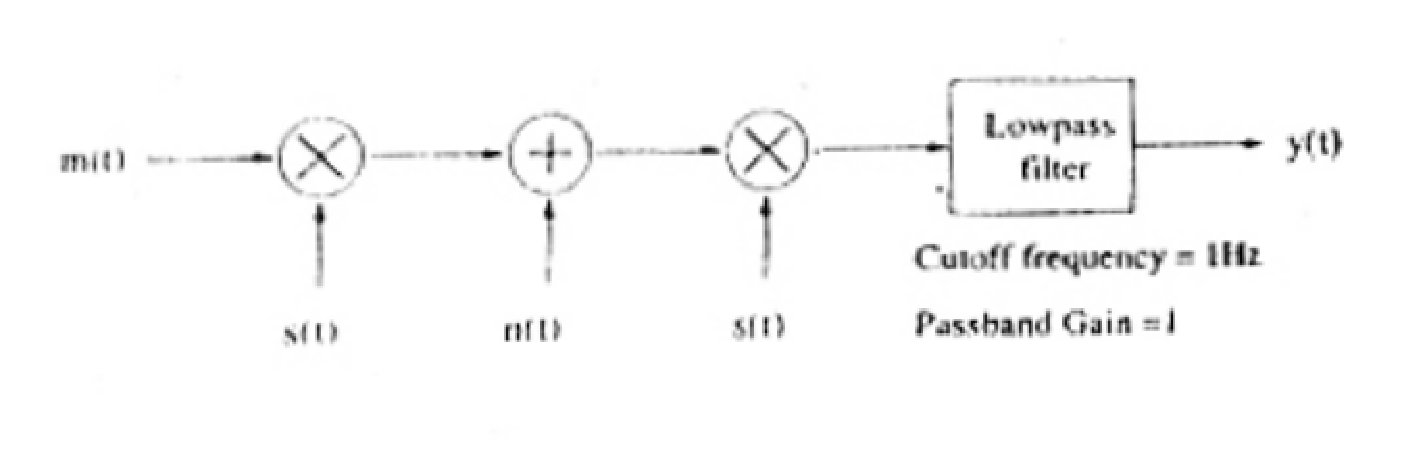
\includegraphics[scale=0.45]{fig20.eps}
\begin{enumerate}[(A)]
\setlength\itemsep{1em}
\item $
\dfrac{sin 2\pi t}{t}
$
\item $
\dfrac{sin 2\pi t}{t}+\dfrac{sin 2\pi t}{t}cos(3 \pi t)
$
\item $
\dfrac{sin 2\pi t}{t}+\dfrac{sin 0.5\pi t}{t}cos(1.5 \pi t)
$
\item $
\dfrac{sin 2\pi t}{t}+\dfrac{sin \pi t}{t}cos(0.75 \pi t)
$

\end{enumerate}

\item A signal $x(t)=100 cos(24 \pi \times 10^{3}t)$ is ideally sampled with a sampling period of 50$\mu$sec and then passed through an ideal low-pass filter with cutoff frequency of 15 KHz. Which of the following frequencies is/are present at the filter output ?

\begin{enumerate}[(A)]
\begin{multicols}{2}
\setlength\itemsep{1em}
\item 
12 KHz only

\item 8 KHz only
\item 12 KHz and 9 KHz


\item 12 KHz and 8 KHz


\end{multicols}
\end{enumerate}

\item The Fourier series expansion of a real periodic signal with fundamental frequency $f_0$ is given by $g_p(t)=\sum\limits_{n=-\infty}^{+\infty} c_n e^{j2\pi n f_0 t}$ is is given that $C_3=3+j5$.Then $C_{-3}$ is
\begin{enumerate}[(A)]
\begin{multicols}{2}
\setlength\itemsep{1em}
\item $
5+j3
$
\item $
-3-j5
$
\item $
-5-j3
$
\item $
3-j5
$
\end{multicols}
\end{enumerate}

\item Let $x(t)$ be the input to a linear,time-invariant system. The required output is $4x(t-2)$.The transfer function of the system should be
\begin{enumerate}[(A)]
\begin{multicols}{4}
\setlength\itemsep{1em}
\item $
4e^{j4\pi f}
$
\item $
2e^{-j8\pi f}
$
\item $
4e^{-j4\pi f}
$
\item $
2e^{j8\pi f}
$
\end{multicols}
\end{enumerate}


\item Let $x(t)=2cos(800\pi t)+cos(1400\pi t)$,$x(t)$ sampled with the rectangular pulse train shown in figure. The only spectral components (in kHz) present in the sampled signal in the frequency range 2.5 kHz to 3.5 kHz are \\

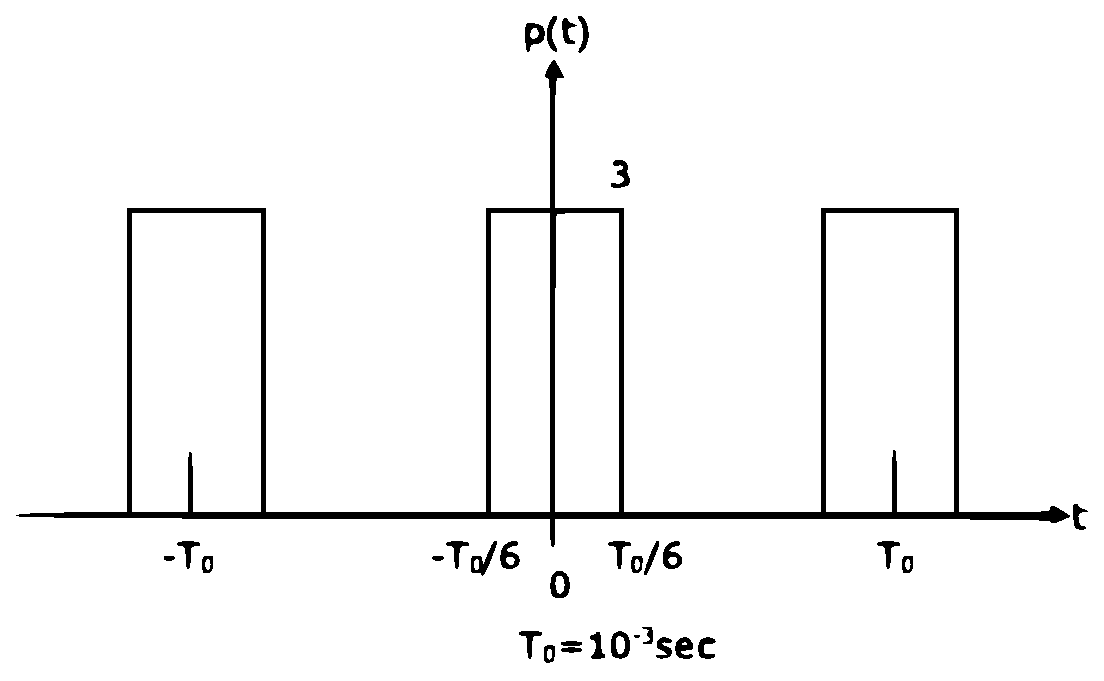
\includegraphics[scale=0.4]{fig2.eps}\\

\begin{enumerate}[(A)]
\begin{multicols}{2}
\setlength\itemsep{1em}
\item $
2.7,3.4
$
\item $
3.3,3.6
$
\item $
2.6,2.7,3.3,3.4,3.6
$
\item $
2.7,3.3
$
\end{multicols}
\end{enumerate}

Data for \textbf{\textit{Q.24-25}} are given below. Solve the problems and choose the correct answers.\newline The system under consideration is an RC low-pass filter (RC-LPF) with R=1.0K$\Omega$ and C=1.0 $\mu$F

\item Let $H(f)$ denote the frequency response of the RC-LPF.Let $f_1$ be the highest frequency such that $0\leq |f| \leq f_1$,$\dfrac{|H(f_1|}{H(0)}\geq 0.95$.Then $f_1$ (in HZ) is
\begin{enumerate}[(A)]
\begin{multicols}{4}
\setlength\itemsep{1em}
\item $
327.8
$
\item $
163.9
$
\item $
52.2
$
\item $
104.4
$
\end{multicols}
\end{enumerate}

\item Let $t_g(f)$ be the group dealy function of the given RC-LPF and $f_2=100 Hz$.Then $t_g(f_2)$ in ms,is\\

\begin{enumerate}[(A)]
\begin{multicols}{4}
\setlength\itemsep{1em}
\item $ 0.717
$
\item $
7.17
$
\item $
71.7$
\item $
4.505$

\end{multicols}
\end{enumerate}


\item The Fourier transform of a conjugate symmetric function is always
\begin{enumerate}[(A)]

\setlength\itemsep{1em}
\item real
\item conjugate anti-symmetric
\item real
\item conjugate symmetric

\end{enumerate}


\item A 1 kHz sinusoidal signal is ideally sampled at 1500 samples/sec and the sampled signal is passed through an ideal low-pass filter with cut-off freuency 800 Hz.The output signal has the frequency ?



\begin{enumerate}[(A)]
\begin{multicols}{2}
\item 0 Hz
\item 0.75 kHz
\item 0.5 kHz
\item 0.25 kHz
\end{multicols}
\end{enumerate}

% ec 2004 61
\item A rectangular pulse train s(t) as shown in figure,is convolved with the signal $cos^{2}(4\pi \times 10^{3})t$.

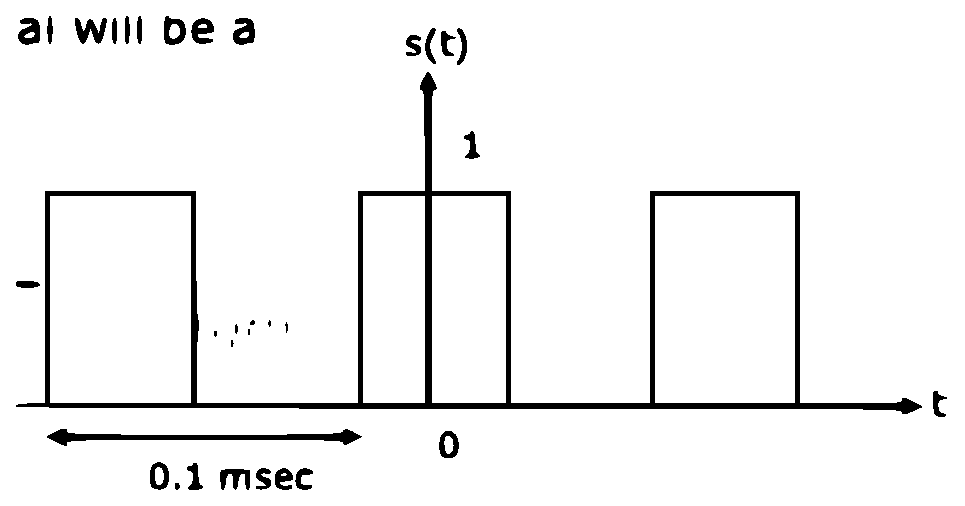
\includegraphics[scale=0.4]{fig3.eps}

\begin{enumerate}[(A)]
\begin{multicols}{2}
\setlength\itemsep{1em}

\item DC
\item 12 kHz sinusoid
\item 8 kHz sinusoid
\item 14 kHz sinusoid
\end{multicols}
\end{enumerate}



\item A causal system having the transfer function $H(s)=\dfrac{1}{s+2}$ is excited with $10u(t)$.The time at which the ouput reaches $99\%$ of its steady state value is
\begin{enumerate}[(A)]
\begin{multicols}{2}
\setlength\itemsep{1em}

\item 2.7 sec
\item 2.5 sec
\item 2.4 sec
\item 2.1 sec

\end{multicols}
\end{enumerate}






% ex 2005 5
\item The function $x(t)$ is shown in figure. Even and odd parts of  a unit-step function $u(t)$ are respectively.\\

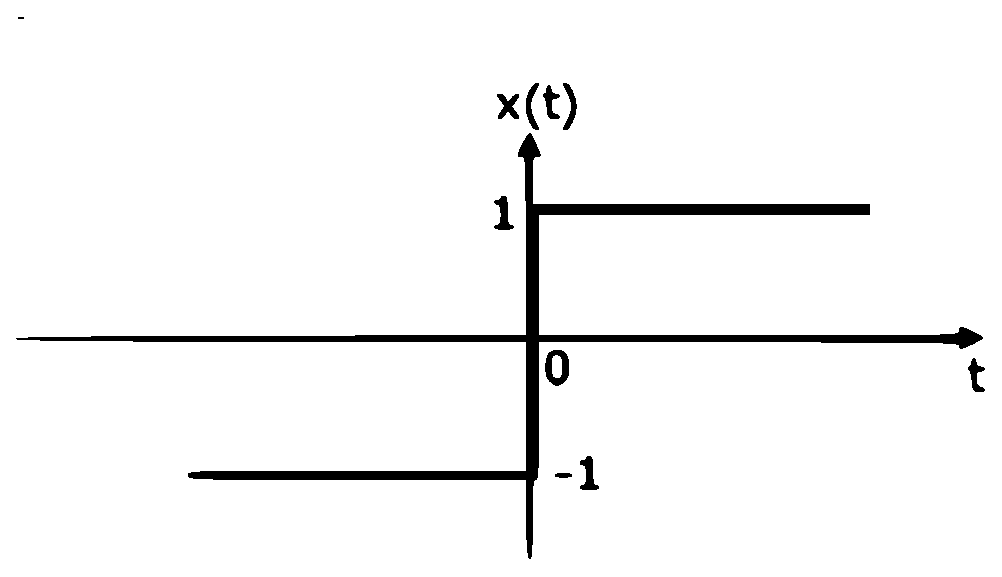
\includegraphics[scale=0.3]{fig4.eps}
\begin{enumerate}[(A)]
\begin{multicols}{2}
\setlength\itemsep{1em}
\item $
\dfrac{1}{2},\dfrac{1}{2}x(t)
$
\item $-\dfrac{1}{2},\dfrac{1}{2}x(t)$
\item $
\dfrac{1}{2},-\dfrac{1}{2}x(t)
$
\item $
-\dfrac{1}{2},-\dfrac{1}{2}x(t)
$
\end{multicols}
\end{enumerate} 



\item The output $y(t)$ of a linear time invariant system is related to its input $x(t)$ by the following equation. $y(t)=0.5x(t-t_d+T)+x(t-t_d)+0.5x(t-t_d-T)$. The filter transfer function $H(w)$ of such a system is given by

\begin{enumerate}[(A)]

\setlength\itemsep{1em}

\item $
(1+coswT)e^{-jwt_d}
$
\item $
(1+0.5coswT)e^{-jwt_d}
$
\item $
(1+coswT)e^{jwt_d}
$
\item $
(1-0.5coswT)e^{-jwt_d}
$

\end{enumerate}


\item For a signal $x(t)$ the Fourier transform is $X(f)$.Then the inverse Fourier transform of $X(3f+2)$ is given by
\begin{enumerate}[(A)]
\begin{multicols}{2}
\setlength\itemsep{1em}

\item $
\dfrac{1}{2} x(\dfrac{1}{2})e^{j3\pi t}
$ 
\item $
3 x(3t)e^{-j4\pi t}
$ 
\item  $
\dfrac{1}{3} x(\dfrac{1}{3})e^{\dfrac{-j4\pi t}{3}}
$ 
\item $
x(3t+2)
$
\end{multicols}
\end{enumerate}

% ec 2005 85
\item \textbf{\textit{(A)}} The Sequence \[
	y(n)=\begin{cases}
		x(\dfrac{n}{2}-1), & \text{for n even }  \\
		0, & \text{odd }\,.
	\end{cases}
\] will be\\
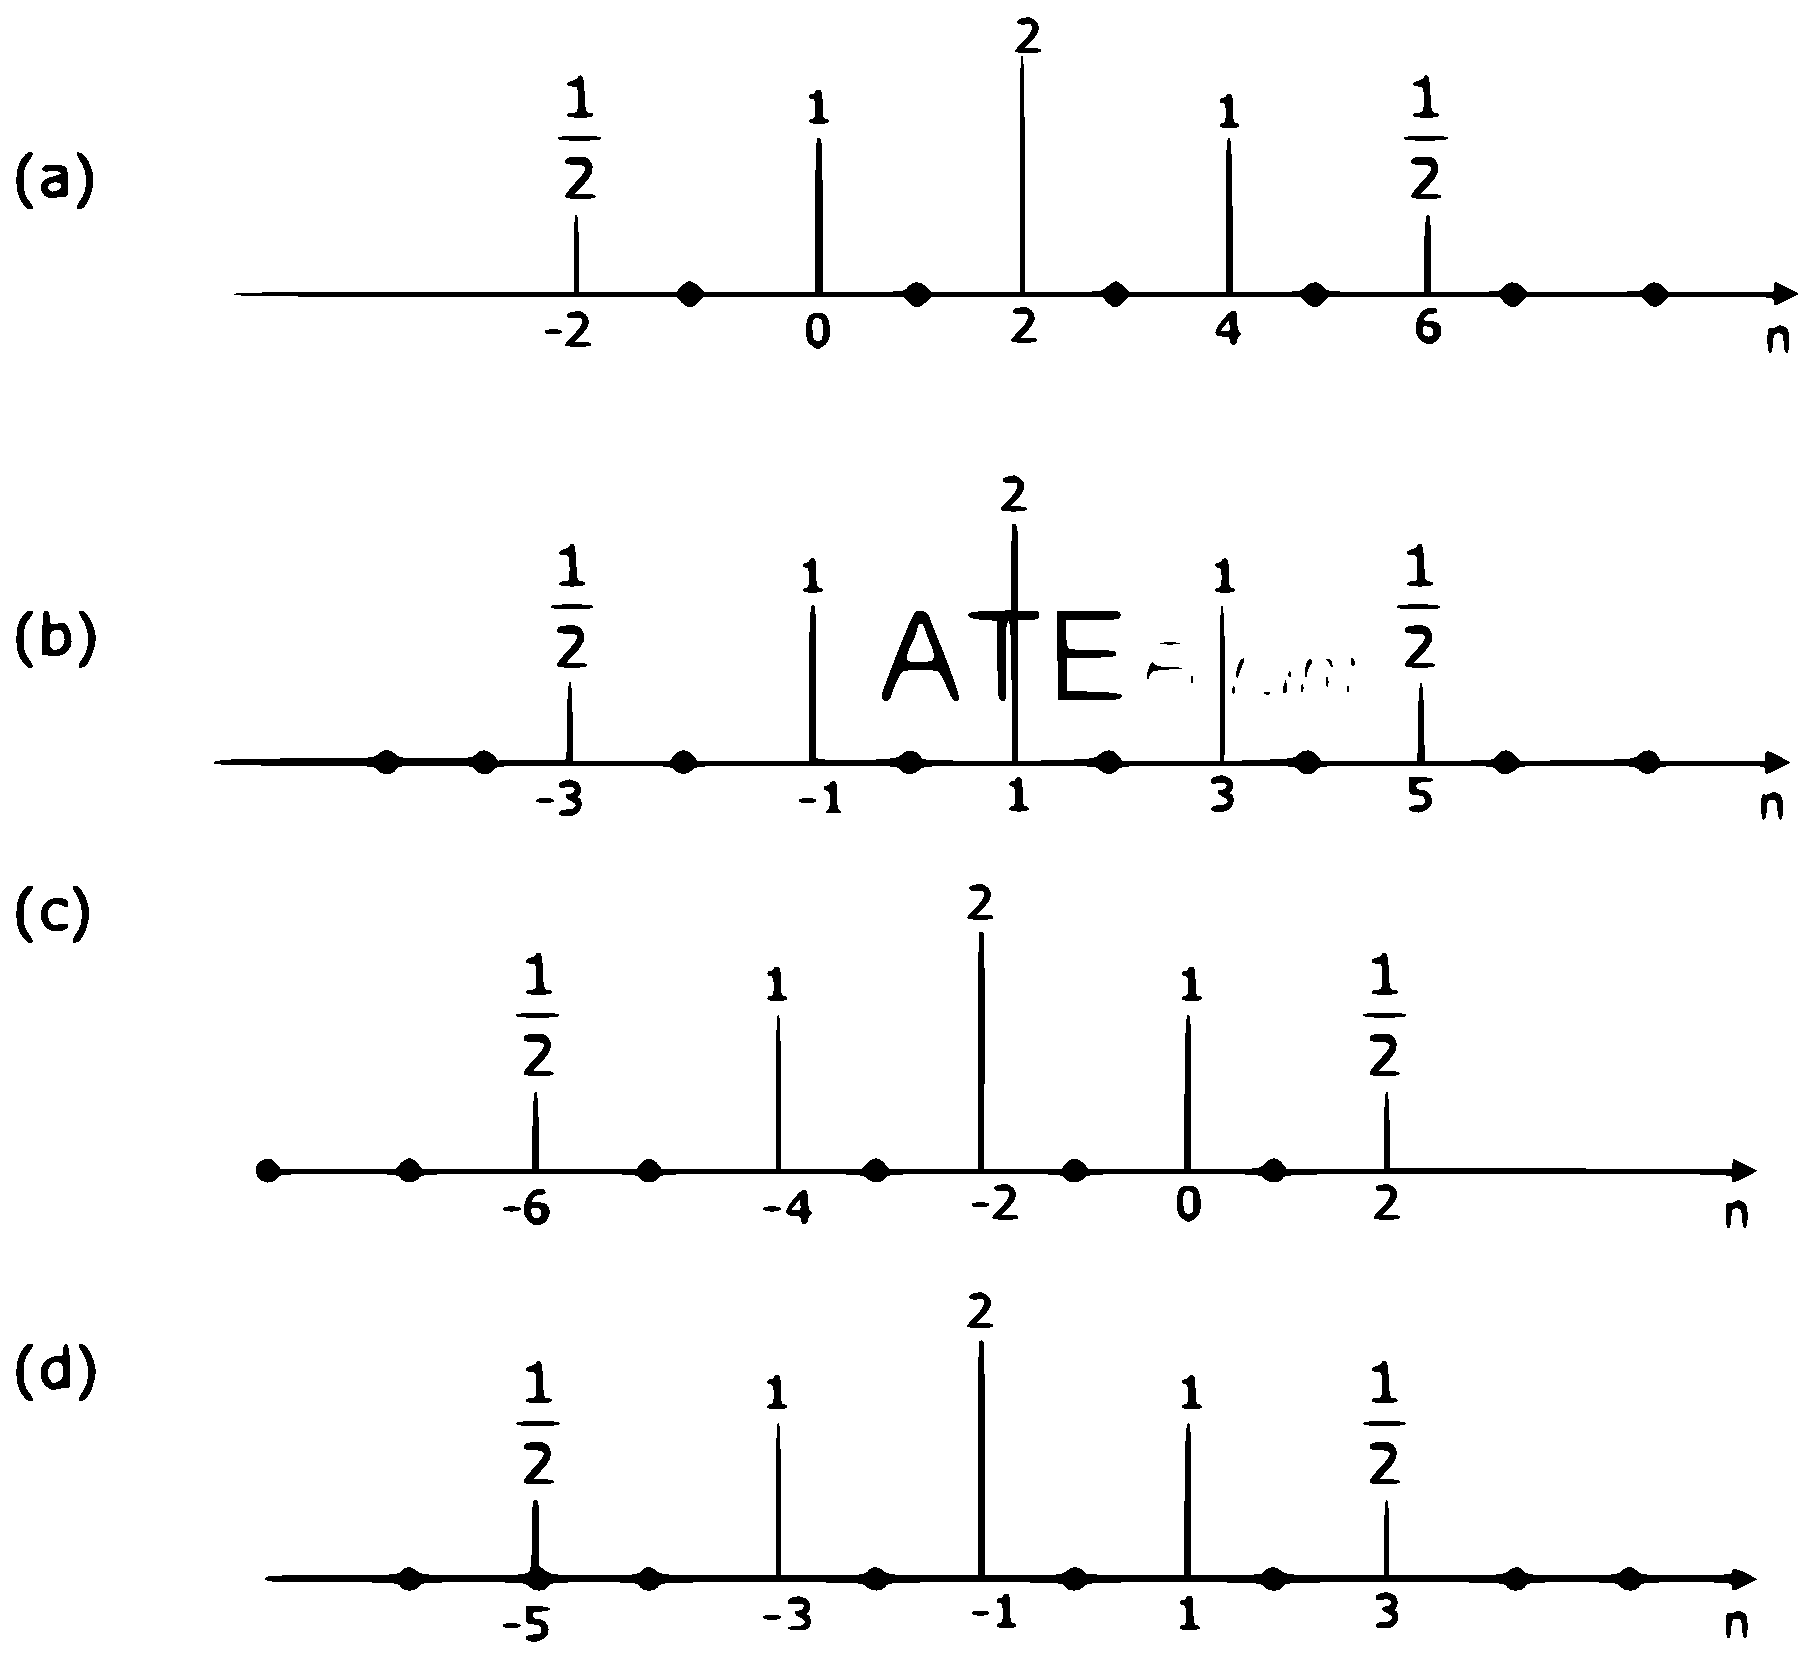
\includegraphics[scale=0.3]{fig6.eps}

\textbf{\textit{(B)}} The Fourier transform of $y(2n)$ will be\\
\begin{enumerate}[(A)]

\setlength\itemsep{1em}

\item $
e^{-2j\omega}[cos 4\omega +2 cos 2\omega +2]
$ 
\item $
[cos2\omega +2 cos\omega +2]
$ 
\item  $
e^{-j\omega}[cos2\omega +2 cos\omega +2]
$ 
\item $
e^{j\omega}[cos2\omega +2 cos\omega +2]
$

\end{enumerate}


\item Let $x(t)\leftrightarrow X(j\omega)$ be Fourier Transform pair.The Fourier Transform of the signal $x(5t-3)$ in terms of $X(j\omega)$ is given as\\
\begin{enumerate}[(A)]

\setlength\itemsep{1em}

\item $
\dfrac{1}{5}e^{\dfrac{-j3\omega}{5}}X(\dfrac{j\omega}{5})
$ 
\item $
\dfrac{1}{5}e^{\dfrac{j3\omega}{5}}X(\dfrac{j\omega}{5})
$ 
\item  $
\dfrac{1}{5}e^{-j3\omega}X(\dfrac{j\omega}{5})
$ 
\item $
\dfrac{1}{5}e^{j3\omega}X(\dfrac{j\omega}{5})
$

\end{enumerate}




\item The dirac delta function $\delta(t)$ is defined as

\begin{enumerate}[(A)]

\setlength\itemsep{1em}

\item \[
	\delta(t)=\begin{cases}
		1, & \text{t=0}  \\
		0, & \text{otherwise }\,.
	\end{cases}
\]
\item \[
	\delta(t)=\begin{cases}
		\infty, & \text{t=0}  \\
		0, & \text{otherwise }\,.
	\end{cases}
\]
\item \[
	\delta(t)=\begin{cases}
		1, & \text{t=0}  \\
		0, & \text{otherwise }\,.
	\end{cases}
\] and \hspace{3mm}$\int_{-\infty}^{+\infty} \delta(t) dt$
\item \[
	\delta(t)=\begin{cases}
		\infty, & \text{t=0}  \\
		0, & \text{otherwise }\,.
	\end{cases}
\] and \hspace{3mm} $\int_{-\infty}^{+\infty} \delta(t) dt$


\end{enumerate}

\item A signal $m(t)$ with bandwidth 500 Hz is first multiplied by a signal $g(t)$ where $g(t)=\sum_{k=-\infty}^{\infty}(-1)^{k}\delta(t-0.5\times 10^{-4}k)$ \newline The resulting signal is then passed through an ideal lowpass filter with bandwidth 1 kHz.The output of the lowpass filter would be:
\begin{enumerate}[(A)]
\begin{multicols}{2}
\setlength\itemsep{1em}

\item $ \delta(t)
$ 
\item $
m(t)
$ 
\item  $
0
$ 
\item $
m(t)\delta(t)
$
\end{multicols}
\end{enumerate}

\item The minimum sampling frequency (in samples/sec) required to reconstruct the following signal from its samples withour distorion. \newline $x(t)=5(\frac{sin 2\pi 1000 t}{\pi t})^{3}+7(\frac{sin 2\pi 1000 t}{\pi t})^{2}$\\
\begin{enumerate}[(A)]
\begin{multicols}{2}
\setlength\itemsep{1em}

\item $2\times 10^{3}$
\item $4\times 10^{3}$
\item $6\times 10^{3}$
\item $8\times 10^{3}$

\end{multicols}
\end{enumerate}

% ec 2006 52
\item A uniformly distributed random variable $x$ with probability density function $f_X(x)=\dfrac{1}{10}(u(x+5)-u(x-5))$ \newline Where $u(.)$ is the unit step function is passed through a transformation given in the figure below.The probability density function of the transformed random variable $Y$ would be\\
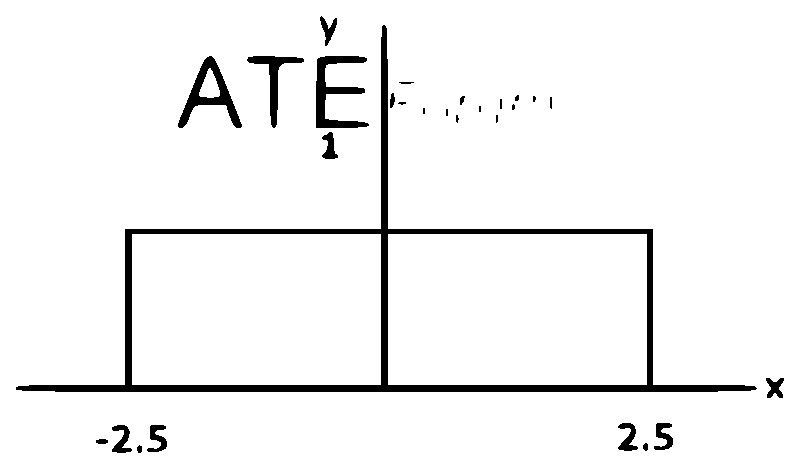
\includegraphics[scale=0.3]{fig7.eps}

\begin{enumerate}[(A)]

\setlength\itemsep{1em}

\item $f_Y(y)=\frac{1}{5}(u(y+2.5)-u(y-2.5))$
\item $f_Y(y)=\frac{1}{2}(\delta(y)-\delta(y-1))$
\item $f_Y(y)=\frac{1}{4}(\delta(y+2.5)-\delta(y-2.5))+\dfrac{1}{2}\delta(y)$
\item $f_Y(y)=\frac{1}{4}(\delta(y+2.5)-\delta(y-2.5))+\dfrac{1}{10}(u(y+2.5))-u(y-2.5)$


\end{enumerate}

\item The 3-dB bandwidth of teh low-pass signal $e^{-t}u(t)$,where $u(t)$ is the unit step function, is given by

\begin{enumerate}[(A)]
\begin{multicols}{2}
\setlength\itemsep{1em}

\item $ \dfrac{1}{2\pi}$ Hz
\item $ \dfrac{1}{2\pi}\sqrt{\sqrt{2}-1}$ Hz
\item $ \infty$
\item 1 Hz

\end{multicols}
\end{enumerate}


\item The unit-step response of a system starting from rest is given by \newline $c(t)=1-e^{-2t} for t \geq 0$
\newline The transfer function of the system is:


\begin{enumerate}[(A)]
\begin{multicols}{2}
\setlength\itemsep{1em}

\item $\dfrac{1}{1+2s}$
\item $\dfrac{2}{2+s}$
\item $\dfrac{1}{2+s}$
\item $\dfrac{2s}{1+2s}$

\end{multicols}
\end{enumerate}


\item A Hilbert transformer is a\\

\begin{enumerate}[(A)]
%\begin{multicols}{2}
\setlength\itemsep{1em}

\item non-linear system
\item non-causal system
\item time-varying system
\item low-pass system

%\end{multicols}
\end{enumerate}

\item The frequency response of linear,time-invariant system is given by $H(f)=\dfrac{5}{1+j10\pi f}$. The step response of the system is\\
\begin{enumerate}[(A)]

\setlength\itemsep{1em}

\item $5(1-e^{-5t})u(t)$
\item $5(1-e^{\dfrac{-t}{5}})u(t)$
\item $\dfrac{1}{5}(1-e^{-5t})u(t)$
\item $\dfrac{1}{5}(1-e^{\dfrac{-t}{5}})u(t)$

\end{enumerate}


\item The input and output of a continous time systems are respectively denoted by $x(t)$ and $y(t)$.Which of the following descriptions corresponds to a causal system?\\
\begin{enumerate}[(A)]

\setlength\itemsep{1em}

\item $y(t)=x(t-2)+x(t+4)$
\item $y(t)=(t-4)x(t+1)$
\item $y(t)=(t+4)x(t-1)$
\item $y(t)=(t+5)x(t+5)$


\end{enumerate}


\item The impulse response $h(t)$ of a linear time-invariant continuous time system is described by $h(t)=e^{\alpha t}u(t)+e^{\beta t}u(-t)$,where $u(t)$ denotes the unit step function, and $\alpha$ and $\beta$ are real constants.This system is stable if\\

\begin{enumerate}[(A)]

\setlength\itemsep{1em}

\item $\alpha$ is positive and $\beta$ is positive
\item $\alpha$ is negative and $\beta$ is negative
\item $\alpha$ is positive and $\beta$ is negative
\item $\alpha$ is negative and $\beta$ is positive


\end{enumerate}

\item A linear,time-invariant, causal continuous time system has a rational transfer function with simple poles at s=-2 and s=-4 , and one simple zero at s=-1. A unit step $u(t)$ is applied at the input of the system. At steady state, the output has constant value of 1. The impulse response of this system is\\
\begin{enumerate}[(A)]

\setlength\itemsep{1.5em}

\item $[e^{-2t}+e^{-4t}]u(t)$
\item $[-4e^{-2t}+12 e^{-4t}-e^{-t}]u(t)$
\item $[-4e^{-2t}+12e^{-4t}]u(t)$
\item $[-0.5e^{-2t}+1.5e^{-4t}]u(t)$

\end{enumerate}


\item The signal x(t) is described by
\[
	x(t)=\begin{cases}
		1, & \text{for $-1\leq t \leq 1$}  \\
		0, & \text{otherwise }\,.
	\end{cases}
\]
\begin{enumerate}[(A)]
\begin{multicols}{2}
\setlength\itemsep{1em}

\item $
\pi,2\pi
$
\item $
0.5\pi,1.5\pi
$
\item $
0,\pi
$
\item $
2\pi,2.5\pi
$


\end{multicols}
\end{enumerate}



\item A function is given by $f(t)=sin^{2}t+cos2t.$ Which of the following is true ?

\begin{enumerate}[(A)]

\setlength\itemsep{1em}

\item $f$ has frequnecy components at 0 and $\dfrac{1}{2\pi}$ Hz
\item $f$ has frequnecy components at 0 and $\dfrac{1}{\pi}$ Hz
\item $f$ has frequnecy components at $\dfrac{1}{2\pi}$ and $\dfrac{1}{\pi}$ Hz
\item $f$ has frequnecy components at 0,$\dfrac{1}{2\pi}$ and $\dfrac{1}{2\pi}$ Hz


\end{enumerate}
\item The Fourier series of a real periodic function has only

\begin{enumerate}[(P)]
%\begin{multicols}{2}
\setlength\itemsep{1em}

\item Cosine terms if it is even
\item Sine terms if it is even
\item Cosine terms if it is odd
\item Sine terms if it is odd.

%\end{multicols}
\end{enumerate}
Which of the above statements are correct ?
\begin{enumerate}[(A)]
\begin{multicols}{2}
\setlength\itemsep{1em}

\item P AND S
\item P AND R
\item Q AND S
\item Q AND R

\end{multicols}
\end{enumerate}

% ec 2009 41 pic
\item Consider a system whose input $x$ and output $y$ are related by the equation. 
\newline$y(t)=\int_{-\infty}^{+\infty}x(t-\tau)h(2\tau)d\tau$
Where h(t) is shown in the graph.\\
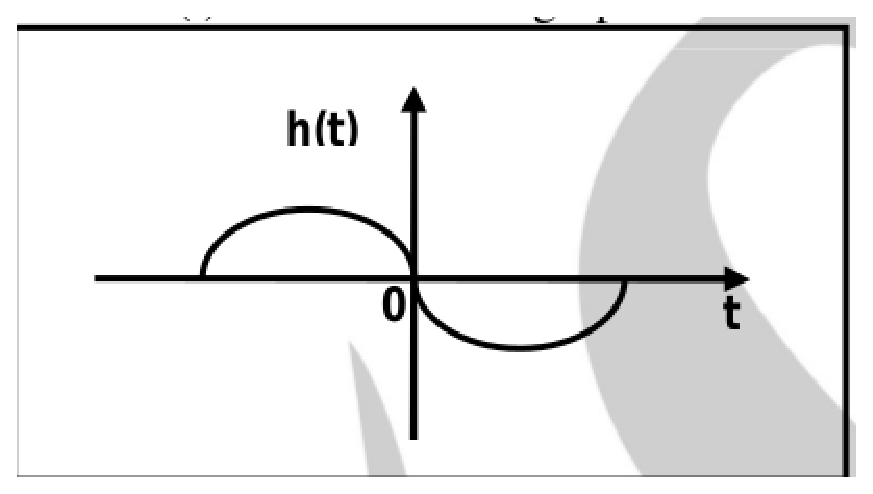
\includegraphics[scale=0.4]{fig9.eps}
\newline Which of the following four properties are possessed by the system ?
\newline \textbf{\textit{BIBO}}:Bounded Input gives Bounded Ouput
\newline \textbf{\textit{Causal}}:The system is Causal.
\newline \textbf{\textit{LP}}:The system is Lowpass.
\newline \textbf{\textit{LTI}}:The system is Linear and Time-Invariant.\\
\begin{enumerate}[(A)]
\begin{multicols}{2}
\setlength\itemsep{1em}

\item Causal, LP
\item BIBO, LTI
\item BIBO, Causal, LTI
\item LP,LTI

\end{multicols}
\end{enumerate}

\item An LTI system having transfer function $\frac{s^{2}+1}{s^{2}+2s+1}$ and input $x(t)=sinx(t)$ is in steady state.The output is sampled at a rate of $\omega_w$ rad/s to obtain the final output $\{y(k)\}$. Which of the following is true ?\\

\begin{enumerate}[(A)]

\setlength\itemsep{1em}

\item y(x) is zero for all sampling frequencies $\omega_s$
\item y(x) is nonzero for all sampling frequencies $\omega_s$
\item y(x) is nonzero for all sampling frequencies $\omega_s>2$, but zero for all $\omega_s<2$
\item y(x) is zero for all sampling frequencies $\omega_s>2$, but nonzero for all $\omega_s<2$

\end{enumerate}

\item The unit step response of an under-damped second order system has steady state value of -2. Which one of the following transfer functions has these properties ?\\


\begin{enumerate}[(A)]

\setlength\itemsep{1em}

\item $\dfrac{-2.24}{s^{2}+2.59s+1.12}$
\item $\dfrac{-3.82}{s^{2}+1.91s+1.91}$
\item $\dfrac{-2.24}{s^{2}-2.59s+1.12}$
\item $\dfrac{-2.24}{s^{2}+2.59s+1.12}$

\end{enumerate}
%ec 2010 2
\item The trigonometric Fourier series for the waveform $f(t)$ shown below contains\\
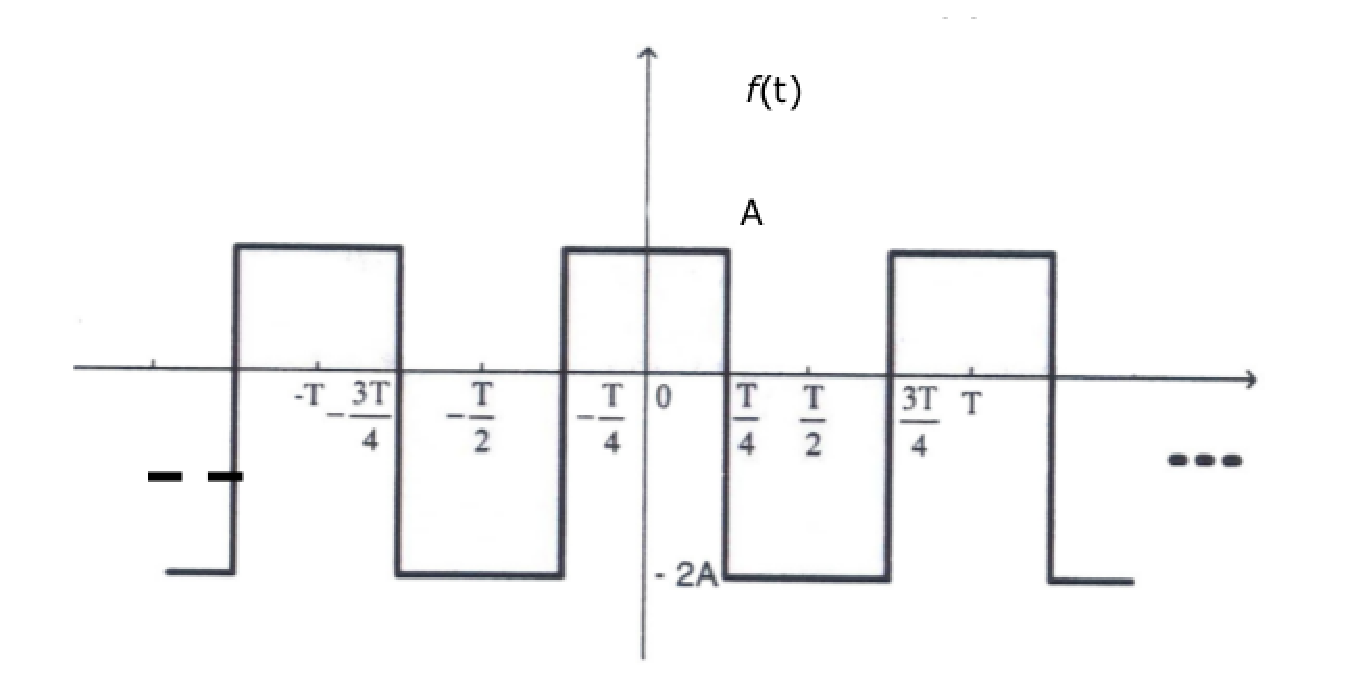
\includegraphics[scale=0.4]{fig10.eps}

\begin{enumerate}[(A)]

\setlength\itemsep{1em}

\item only cosine terms and zero value for the dc component
\item only cosine terms and a positive value for the dc component
\item only cosine terms and a negative value for the dc component
\item only sine terms and a negative for the dc component

\end{enumerate}
\item A system with transfer function $\dfrac{Y(s)}{X(s)}=\dfrac{s}{s+p}$ has an output $y(t)=cos(2t-\dfrac{\pi}{3}$ for the input signal $x(t)=p cos(2t-\dfrac{\pi}{2}$.Then, the system parameter 'p' is


\begin{enumerate}[(A)]

\setlength\itemsep{1em}

\item $\sqrt{3}$
\item $\dfrac{2}{\sqrt{3}}$
\item $1$
\item $\dfrac{\sqrt{3}}{2}$

\end{enumerate}

\item A continous time LTI system is described by $\dfrac{d^{2}y(t)}{dt^{2}}+4\dfrac{dy(t)}{dt}+3y(t)=2\dfrac{dx(t)}{dt}+4x(t)$

\begin{enumerate}[(A)]

\setlength\itemsep{1em}

\item $(e^{t}-e^{3t})u(t)$
\item $(e^{-t}-e^{-3t})u(t)$
\item $(e^{-t}+e^{-3t})u(t)$
\item $(e^{t}+e^{3t})u(t)$

\end{enumerate}


\item The Nyquist sampling rate for the signal $s(t)=\dfrac{sin(500\pi t)}{\pi t}\times \dfrac{sin(700\pi t)}{\pi t}$ is given by 

\begin{enumerate}[(A)]
\begin{multicols}{2}
\setlength\itemsep{1em}

\item 400 Hz
\item 600 Hz
\item 1200 Hz
\item 1400 Hz
\end{multicols}
\end{enumerate}

\item If the unit step response of a network is $1-e^{-\alpha t}$, then its unit impulse response

\begin{enumerate}[(A)]
%\begin{multicols}{4}
\setlength\itemsep{1em}

\item $\alpha e^{-\alpha t}$
\item $\alpha^{-1} e^{-\alpha t}$
\item $(1-\alpha^{-1}) e^{-\alpha t}$
\item $(1-\alpha) e^{-\alpha t}$
%\end{multicols}
\end{enumerate}

\item The trigonometric Fourier series of an even function does not have the
\begin{enumerate}[(A)]
%\begin{multicols}{4}
\setlength\itemsep{1em}

\item dc term
\item cosine terms
\item sine terms
\item odd harmonic terms
%\end{multicols}
\end{enumerate}

\item An input $x(t)=e^{-2t}u(t)+\delta(t-6)$ is applied to an LTI system with impulse response $h(t)=u(t)$.The output is
\begin{enumerate}[(A)]
%\begin{multicols}{4}
\setlength\itemsep{1em}

\item $[1-e^{-2t}]u(t)+u(t+6)$
\item $[1-e^{-2t}]u(t)+u(t-6)$
\item $0.5[1-e^{-2t}]u(t)+u(t+6)$
\item $0.5[1-e^{-2t}]u(t)+u(t-6)$
%\end{multicols}
\end{enumerate}



\item The systems with impulse responses $h_1(t)$ and $h_2(t)$ are connected in cascade. Then the overall impulse response of the cascaded system is given by
\begin{enumerate}[(A)]
%\begin{multicols}{2}
\setlength\itemsep{1em}

\item product of $h_1(t)$ and $h_2(t)$
\item sum of $h_1(t)$ and $h_2(t)$
\item convolution of $h_1(t)$ and $h_2(t)$
\item Substraction of $h_2(t)$ and $h_1(t)$
%\end{multicols}
\end{enumerate}


\item A band-limited signal with a maximum frequency of 5 kHz is to be sampled. According to the sampling theorem, the sampling frequency which is not valid is
\begin{enumerate}[(A)]

\begin{multicols}{2}
\setlength\itemsep{1em}

\item 5 kHz
\item 12 kHz
\item 15 kHz
\item 20 kHz
\end{multicols}
\end{enumerate}

%ec  2013 21
\item Assuming zero initial condition, the response $y(t)$ of the system given below to a unit step input $u(t)$ is\\
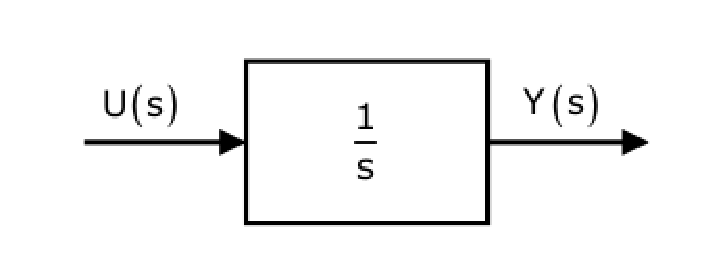
\includegraphics[scale=0.4]{fig12.eps}
\begin{enumerate}[(A)]

\begin{multicols}{2}
\setlength\itemsep{1em}

\item $u(t)$
\item $tu(t)$
\item $\frac{t^{2}}{2}u(t)$
\item $e^{-t} u(t)$
\end{multicols}
\end{enumerate}

\item A system is described by the differential equation $\frac{d^{2}y}{dt^{2}}+5\frac{dy}{dt}+6y(t)=x(t)$. Let x(t)  be a rectangular pulse given by\[
	x(t)=\begin{cases}
		1, & \text{$0<t<2$}  \\
		0, & \text{otherwise }\,.
	\end{cases}
\] Assuming that $y(0)=0$ and $\frac{dy}{dt}=0$ at t=0, the Laplace transform of $y(t)$ is

\begin{enumerate}[(A)]

\begin{multicols}{2}
\setlength\itemsep{1em}

\item $\frac{e^{-2s}}{s(s+2)(s+3)}$
\item $\frac{1-e^{-2s}}{s(s+2)(s+3)}$
\item $\frac{e^{-2s}}{(s+2)(s+3)}$
\item $\frac{1-e^{-2s}}{(s+2)(s+3)}$
\end{multicols}
\end{enumerate}










\item The impulse response of a system is $h(t)=tu(t)$.For an input $u(t-1)$,the output is
\begin{enumerate}[(A)]

%\begin{multicols}{2}
\setlength\itemsep{1em}

\item $\frac{t^{2}}{2}u(t)$
\item $\frac{t\times (t-1)}{2}u(t-1)$
\item $\frac{(t-1)^{2}}{2}u(t-1)$
\item $\frac{t^{2}-1}{2}u(t-1)$
%\end{multicols}
\end{enumerate}

\item The value of the integral $\int_{-\infty}^{+\infty} sinc^{2}(5t) dt$ is \underline{\hspace{1cm}}

%ec 2014 papr2 19
\item Consider the periodic square wave in the figure shown.
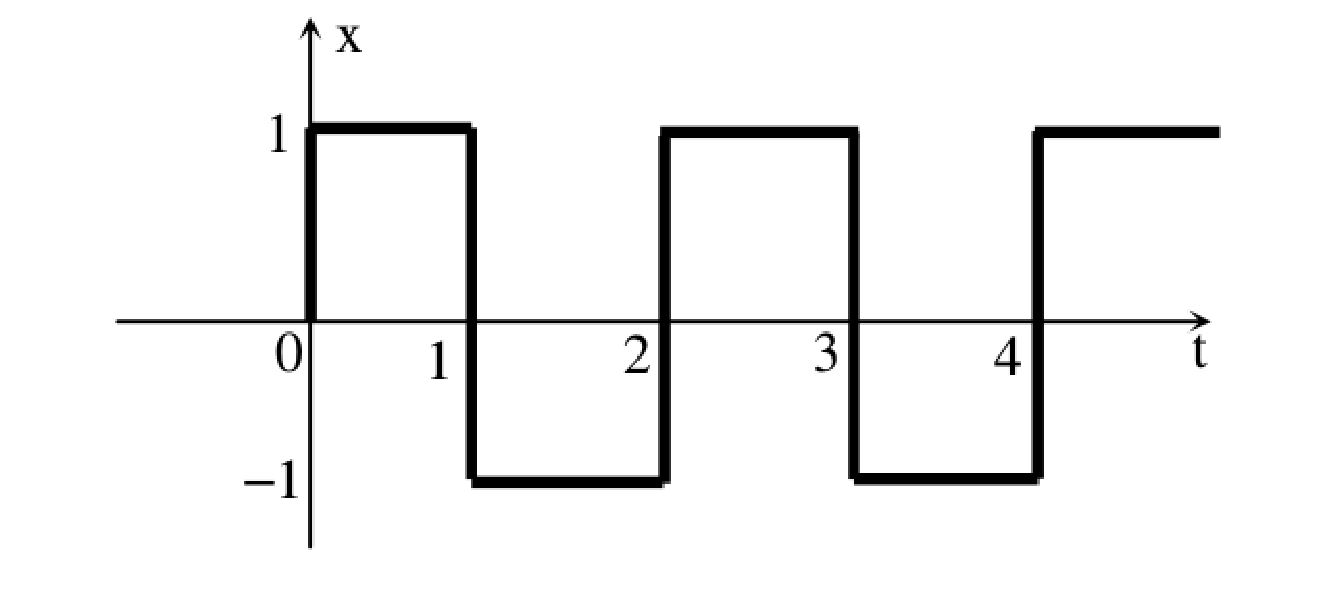
\includegraphics[scale=0.4]{fig13.eps}
\newline The ratio of the power in the $7^{th}$ harmonic to the power in the $5^{th}$ harmonic for this waveform is closest in value to \underline{\hspace{2cm}}\\






% set1 2015 18
\item The waveform of a periodic signal $x(t)$ is shown in the figure.\\
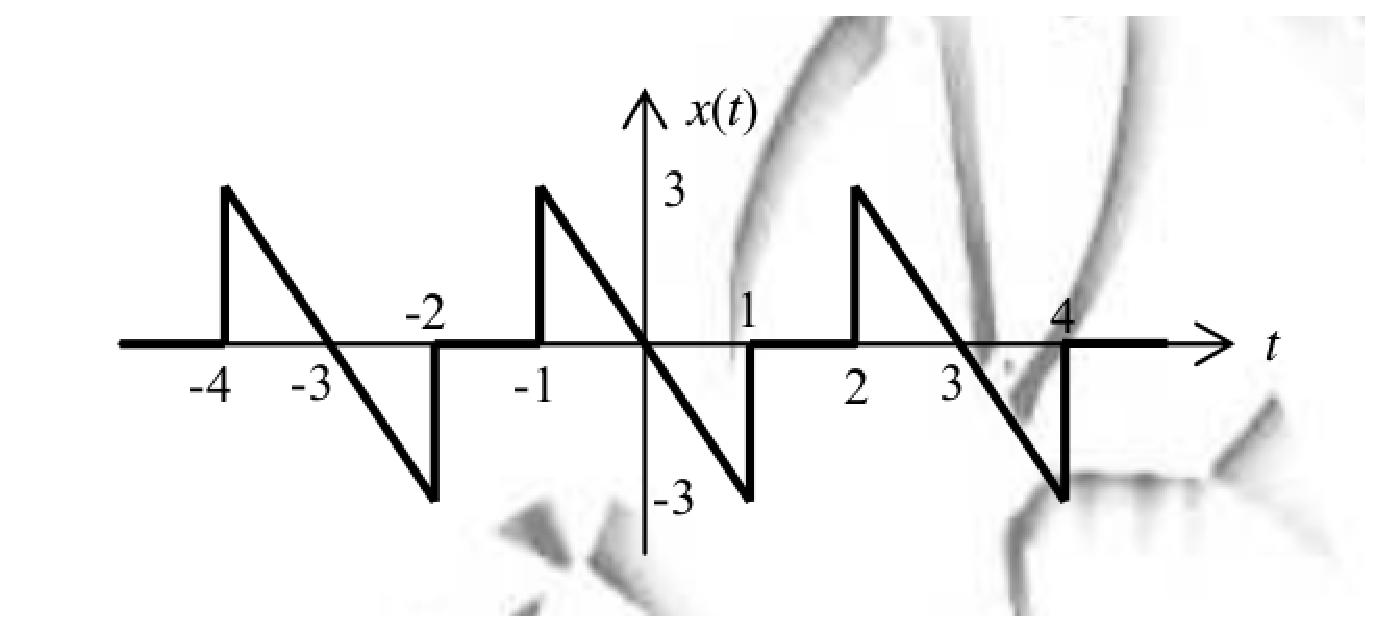
\includegraphics[scale=0.4]{fig14.eps}
\newline A signal $g(t)$ is defined by $g(t)=x(\frac{t-1}{2})$. The average power of $g(t)$ is \underline{\hspace{2cm}}\\


\item Consider the signal $s(t)=m(t)cos(2\pi f_c t)+\hat{m}(t)sin(2\pi f_c t)$ where $\hat{m}(t)$ denotes the Hilbert transform of $m(t)$ and the bandwidth of $m(t)$ is very small compared to $f_c$.The signal $s(t)$ is a

\begin{enumerate}[(A)]

%\begin{multicols}{2}
\setlength\itemsep{1em}

\item high-pass signal
\item low-pass signal
\item band-pass signal
\item double sideband suppressed carrier signal
%\end{multicols}
\end{enumerate}





\item A continuous-time sinusoid of frequency 33 Hz is multiplied with a periodic Dirac impulse train of frequency 46 Hz. The resulting signal is passed through an ideal analog low-pass filter with a cutoff frequency of 23 Hz. The fundamental frequency (in Hz) of the output is \underline{\hspace{2cm}}

% 51 2015 set1
\item In the system shown in Figure(a), $m(t)$ is a low-pass signal with bandwidth $W$ Hz. The frequency response of the band-pass filter $H(f)$ is shown in Figure(b). If it is described that the output signal $z(t)=10x(t)$, the maximum value of $W$ (in Hz) should be strictly less than \underline{\hspace{2cm}}\\
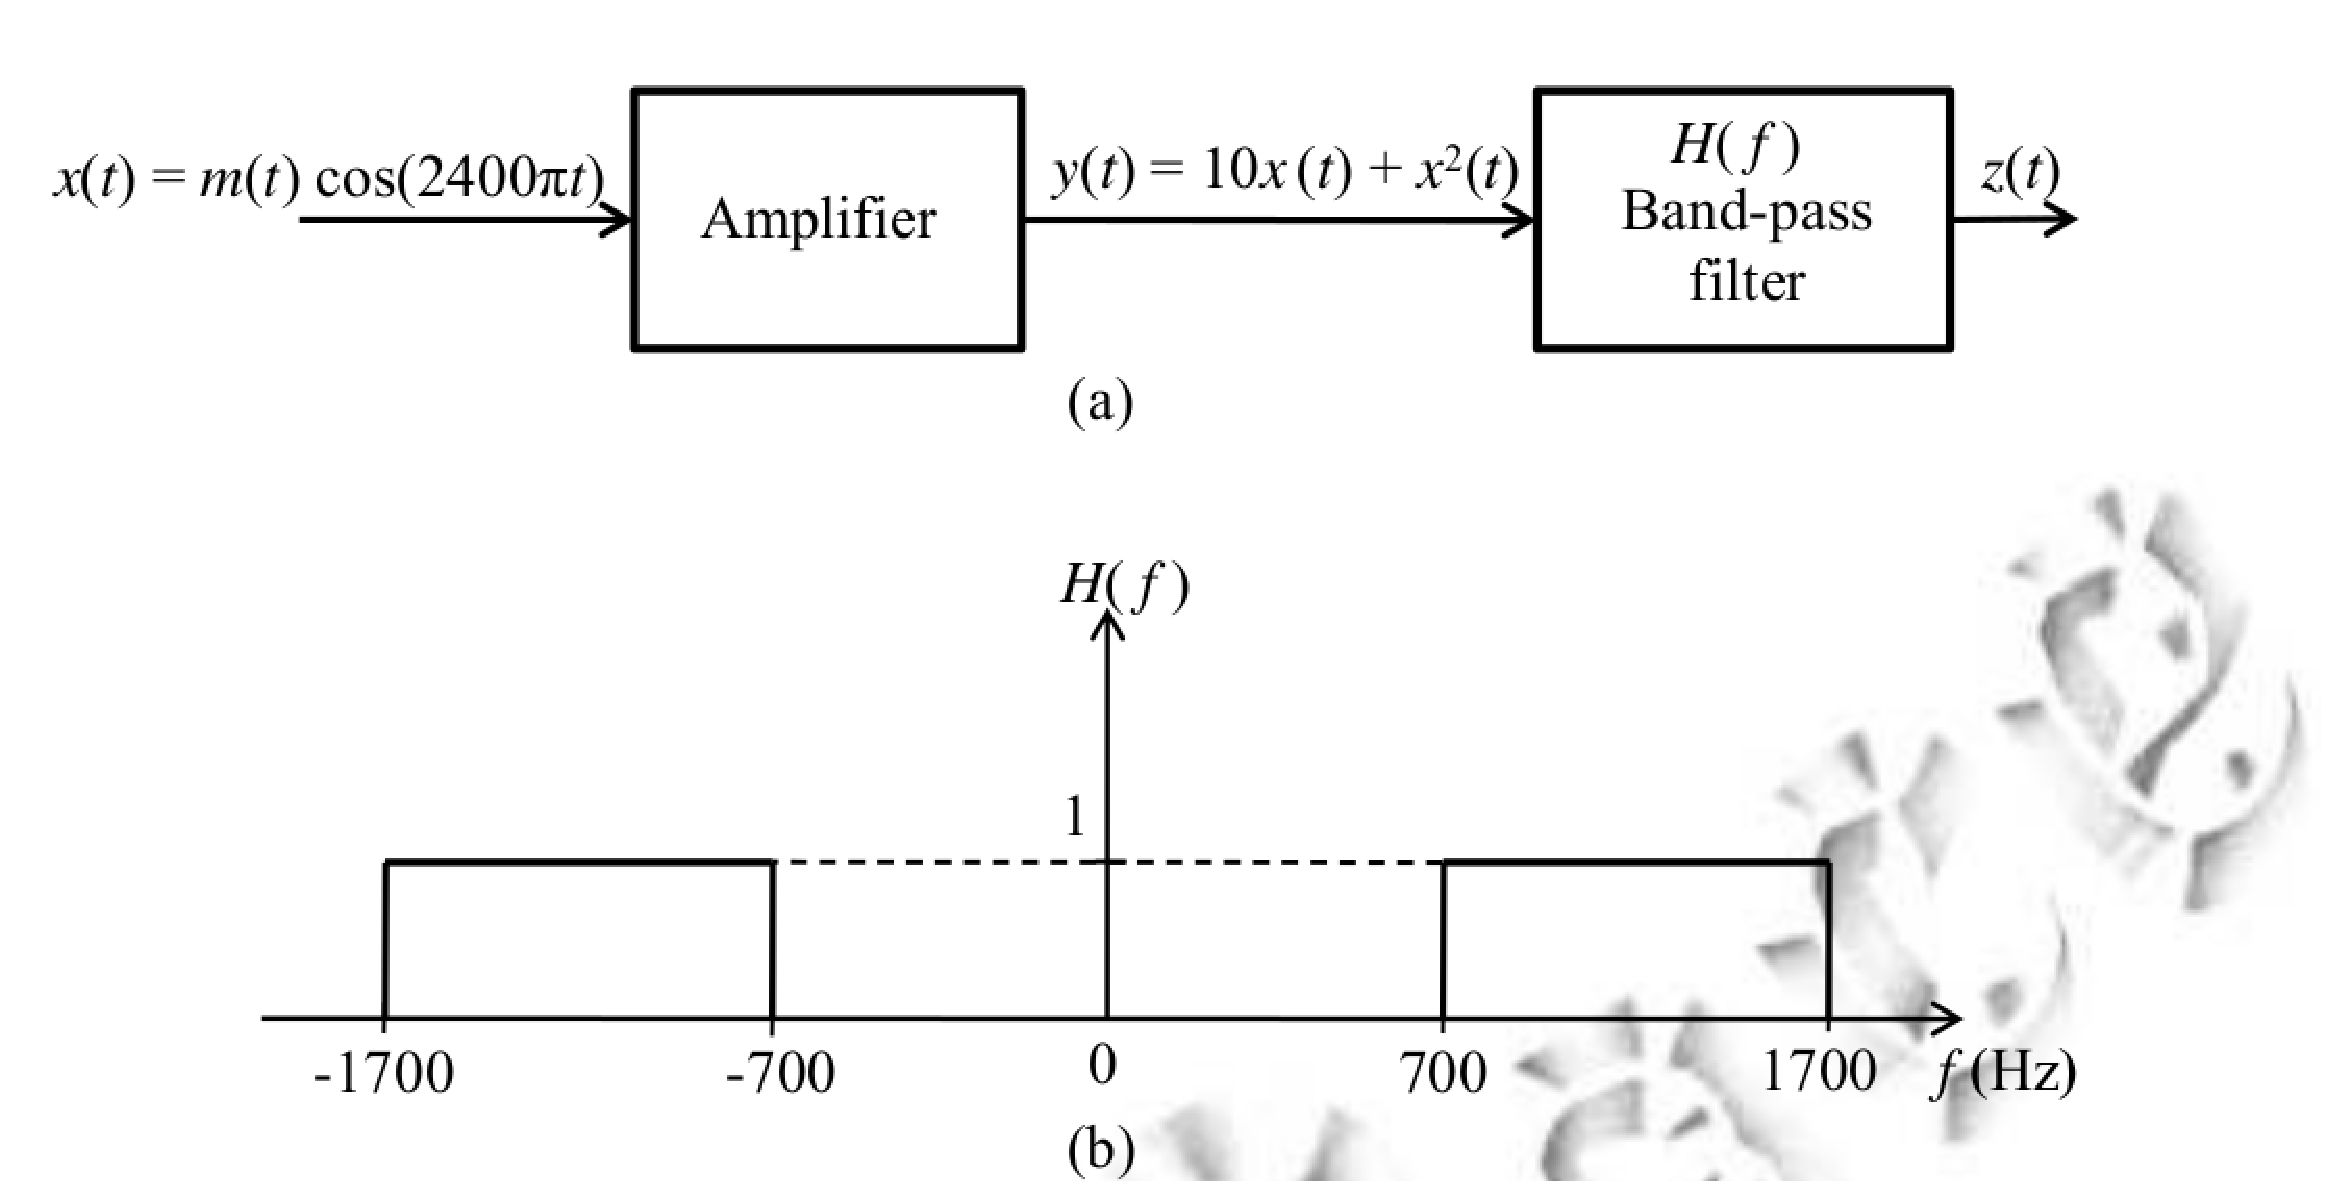
\includegraphics[scale=0.2]{fig17.eps}


Data for \textbf{\textit{Questions}} given below.\newline
\hspace{1em}The impulse response $h(t)$ of a linear time invariant continuous time system is given by $h(t)=e^{-2t}u(t)$, where $u(t)$ denotes the unit step function.\newline
\item The frequency response $H(\omega)$ of this system in terms of angular frequency $\omega$ is give by $H(\omega)$ 



\begin{enumerate}[(A)]
\begin{multicols}{2}
\setlength\itemsep{1em}

\item $
\dfrac{1}{1+j2\omega}
$
\item $
\dfrac{sin(\omega)}{\omega}
$
\item $
\dfrac{1}{2+j\omega}
$
\item $
\dfrac{j\omega}{2+j\omega}
$

\end{multicols}
\end{enumerate}



\item The output of this system to the sinusoidal input $x(t)=2cos(2t)$ $\forall t$, is

\begin{enumerate}[(A)]

\setlength\itemsep{1em}

\item 0
\item $2^{-0.25}cos(2t-0.125\pi)$
\item $2^{-0.5}cos(2t-0.125\pi)$.
\item $2^{-0.5}cos(2t-0.25\pi)$


\end{enumerate}

\item A system described by a linear,constant coefficient, ordinary, first order differential equation has an exact solution given by $y(t)$ for $t>0$,when the forcing function is $x(t)$ and the initial condistion is $y(0)$.If one wishes to modify the system so that the solution becomes $-2y(t)$ for $t>0$, we need to
\begin{enumerate}[(A)]

%\begin{multicols}{2}
\setlength\itemsep{2mm}

\item change the initial condition to $-y(0)$ and the forcing function to $2x(t)$
\item change the initial condition to $2y(0)$ and the forcing function to $-x(t)$
\item change the initial condition to $j\sqrt{2y(0)}$ and the forcing function to $j\sqrt{x(t)}$
\item change the initial condition to $-2y(0)$ and the forcing function to $-2x(t)$
%\end{multicols}
\end{enumerate}

%ec paper 2014 52
\item In the figure,$M(f)$ is the Fourier transform of the message signal,$m(t)$ where A=100 Hz and B=40 Hz. Given $v(t)=cos(2\pi f_c t)$ and $w(t)=cos(2\pi (f_c +A))$, where $f_c > A$ The cutoff frequencies of the both filters are \underline{\hspace{2cm}} $f_c$\\
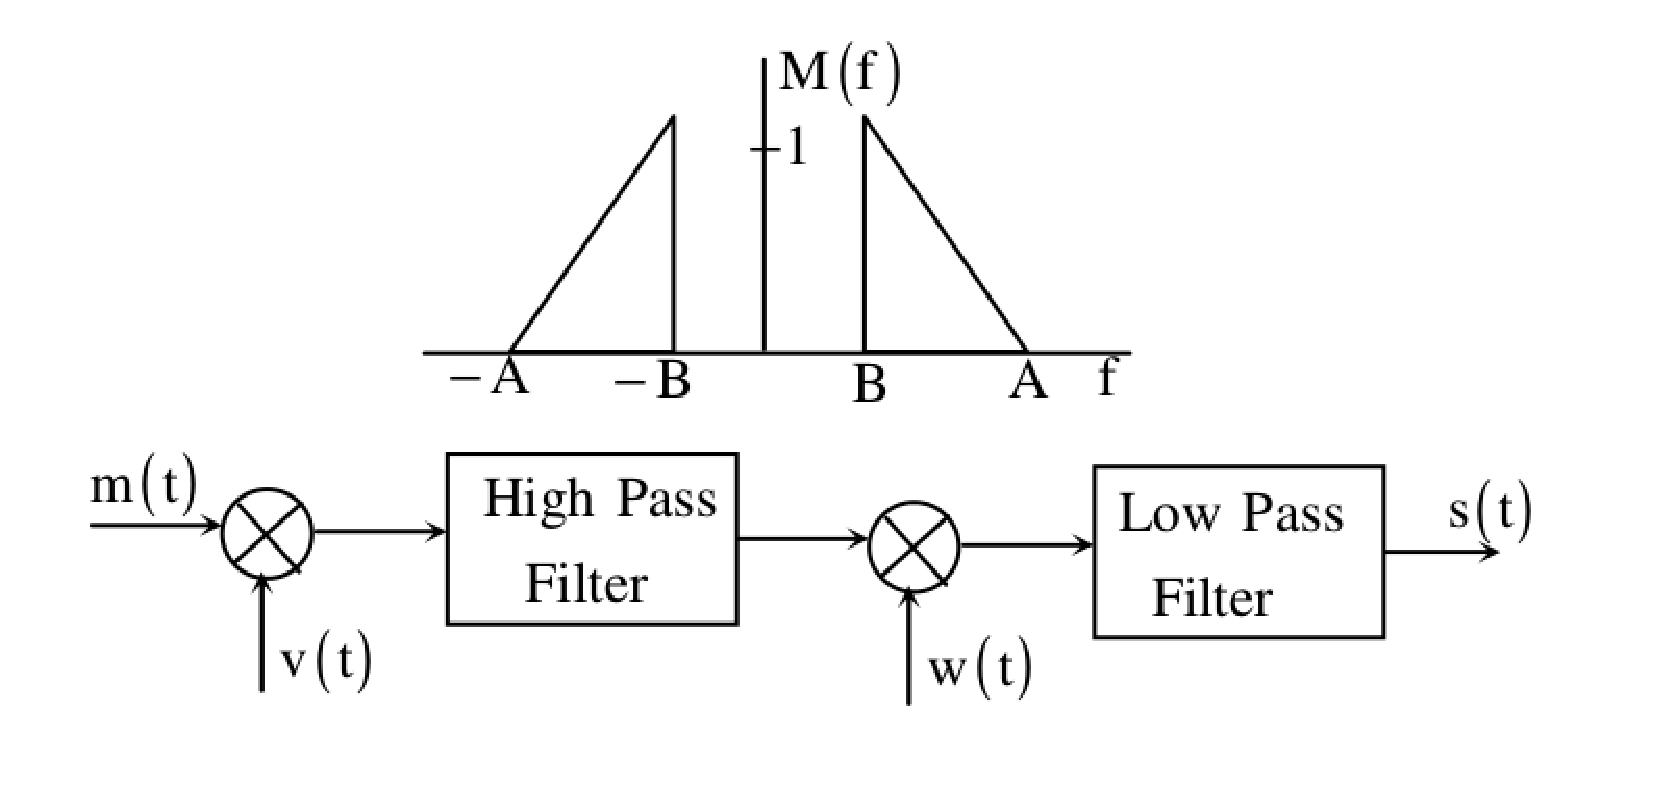
\includegraphics[scale=0.3]{fig18.eps}


\item The result of the convolution $x(-t)*\delta(-t-t_0)$ is
\begin{enumerate}[(A)]

\begin{multicols}{2}
\setlength\itemsep{1em}

\item $x(t+t_0)$
\item $x(t-t_0)$
\item $x(-t+t_0)$
\item $x(-t-t_0)$
\end{multicols}
\end{enumerate}

\end{enumerate}


\end{document}
